\documentclass[12pt]{report}
\usepackage{graphicx}
\usepackage[utf8]{inputenc}
\usepackage[spanish]{babel}
\usepackage{setspace}
\usepackage{geometry}
\usepackage{titlesec}
\usepackage{times}
\usepackage{mathptmx} % Use mathptmx instead of times
\usepackage{fancyhdr}
\usepackage{float}
\usepackage{pdfpages}



% Configuración de márgenes
\geometry{
    top=2.5cm,
    left=3cm,
    right=3cm,
    bottom=2.5cm
}

% Configuración de interlineado
\onehalfspacing

% Configuración de títulos y subtítulos
\titleformat{\chapter}[display]
  {\normalfont\bfseries\centering}{}{0pt}{\fontsize{14}{16}\selectfont}
\titleformat{\section}
  {\normalfont\bfseries}{\thesection}{1em}{\fontsize{12}{14}\selectfont}
\titleformat{\subsection}
  {\normalfont\bfseries}{\thesubsection}{1em}{\fontsize{12}{14}\selectfont}


% Configuración de pie de página
  \fancyhf{}
\fancyfoot[R]{\thepage}
\pagestyle{fancy}
\fancypagestyle{plain}{
  \fancyhf{}
  \fancyfoot[R]{\thepage}
}

  \begin{document}
  \pagenumbering{roman}
%----- PORTADA ----
\setlength{\hoffset}{27 pt} % 1 (Para centrar más la portada)
\begin{titlepage}
{\centering
{\fontfamily{ptm}\scshape\bfseries\fontsize{29.16}{34.992}\selectfont Universidad de Guadalajara \par}
\vspace{0.5cm}
{\scshape\Large Centro Universitario de los Lagos \par}
\vspace{1cm}
{\scshape\Large División de Estudios de la Biodiversidad e innovación Tecnológica \par}
\vspace{1cm}
{\graphicspath{{imagenes/Portada}} %ruta de las imagenes

\includegraphics[width=0.3\textwidth]{image.png}\par}
\vspace{1cm}
% Título
{\scshape\large\bfseries Practica 5: Función LATCH/UNLATCH (SET/RESET) \par}
\vspace{0.5cm}
% Materia
{\large \textbf{Materia:} \\Controladores Lógicos Programables\par}
\vfill
% Estudiante
{\large \textbf{Presenta:} \\Oscar Iván Moreno Gutiérrez \#220942754
\\Maximiliano Frias Campos \#217488066
\par}
\vfill
% Profesor
{\large \textbf{Profesor:} \\Dr. Afanador Delgado Samuel Mardoqueo \par}
\vfill
\vfill
% Fecha
\begin{flushright}
  {\normalsize \textbf {Fecha:} \\ \today}
\end{flushright}
\vfill}
{\large  \par}
\end{titlepage}
%----- FIN DE PORTADA ----

%----- ÍNDICE GENERAL ----
\tableofcontents
\newpage

%----- PALABRAS CLAVE ----
\pagenumbering{arabic}
\chapter*{Palabras Clave}

\addcontentsline{toc}{chapter}{Palabras Clave}
\begin{itemize}
  \item \textbf{LATCH/UNLATCH (SET/RESET):} Funciones utilizadas en la programación de PLCs para mantener el estado de una salida hasta que se cumpla una condición específica para cambiar dicho estado.
  \item \textbf{Circuito Predominante SET:} Un circuito que mantiene una salida activada hasta que se cumpla una condición específica para desactivarla.
  \item \textbf{Circuito Predominante RESET:} Un circuito que desactiva una salida previamente activada por un circuito SET, asegurando que las operaciones se realicen de manera controlada.
\end{itemize}

%\begin{itemize}

%\end{itemize}
\newpage

%----- OBJETIVO ----
\chapter*{Objetivo}
\addcontentsline{toc}{chapter}{Objetivo}
  Comprender y aplicar la función LATCH/UNLATCH, también conocida como SET/RESET, como alternativa simplificadora del circuito de autoenergización.
\newpage

%----- CONTENIDO ----
\chapter{Contenido}
\section{¿Qué es LATCH/UNLATCH?}
La función LATCH/UNLATCH, también conocida como SET/RESET, es una técnica utilizada en la programación de Controladores Lógicos Programables (PLC) para mantener el estado de una salida hasta que se cumpla una condición específica para cambiar dicho estado. Esta función es una alternativa simplificada al circuito de autoenergización.

\subsection{Funcionamiento de LATCH}
La función LATCH (o SET) se utiliza para activar una salida y mantenerla en ese estado hasta que se ejecute una función UNLATCH (o RESET). Cuando se activa la condición de LATCH, la salida se establece en un estado alto (encendido) y permanece en ese estado incluso si la condición de activación desaparece.

\subsection{Funcionamiento de UNLATCH}
La función UNLATCH (o RESET) se utiliza para desactivar una salida que ha sido activada por una función LATCH. Cuando se activa la condición de UNLATCH, la salida se establece en un estado bajo (apagado) y permanece en ese estado hasta que se ejecute otra función LATCH.



\section{Materiales}
Para la realización de esta práctica se utilizaron los siguientes materiales:

\begin{itemize}
  \item \textbf{Aplicación con picosoft:} Software utilizado para la simulación y programación de PLCs.
  \item \textbf{PLC:} Controlador Lógico Programable utilizado para la implementación del circuito.
  \item \textbf{Botonera:} Dispositivo que contiene los botones de arranque y paro.
  \item \textbf{Botones:} Componentes individuales de la botonera utilizados para controlar el circuito.
\end{itemize}

\section{Procedimiento}
\begin{enumerate}
  \item Declaramos las variables de nuestro circuito.
        \begin{figure}[H]
          \centering
          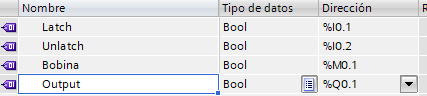
\includegraphics[width=0.5\textwidth]{screenshots/variables.png}
          \caption{Variables del circuito}
          \label{fig:variables}
        \end{figure}
  \item Creamos el primer circuito dominante SET.
        \begin{figure}[H]
          \centering
          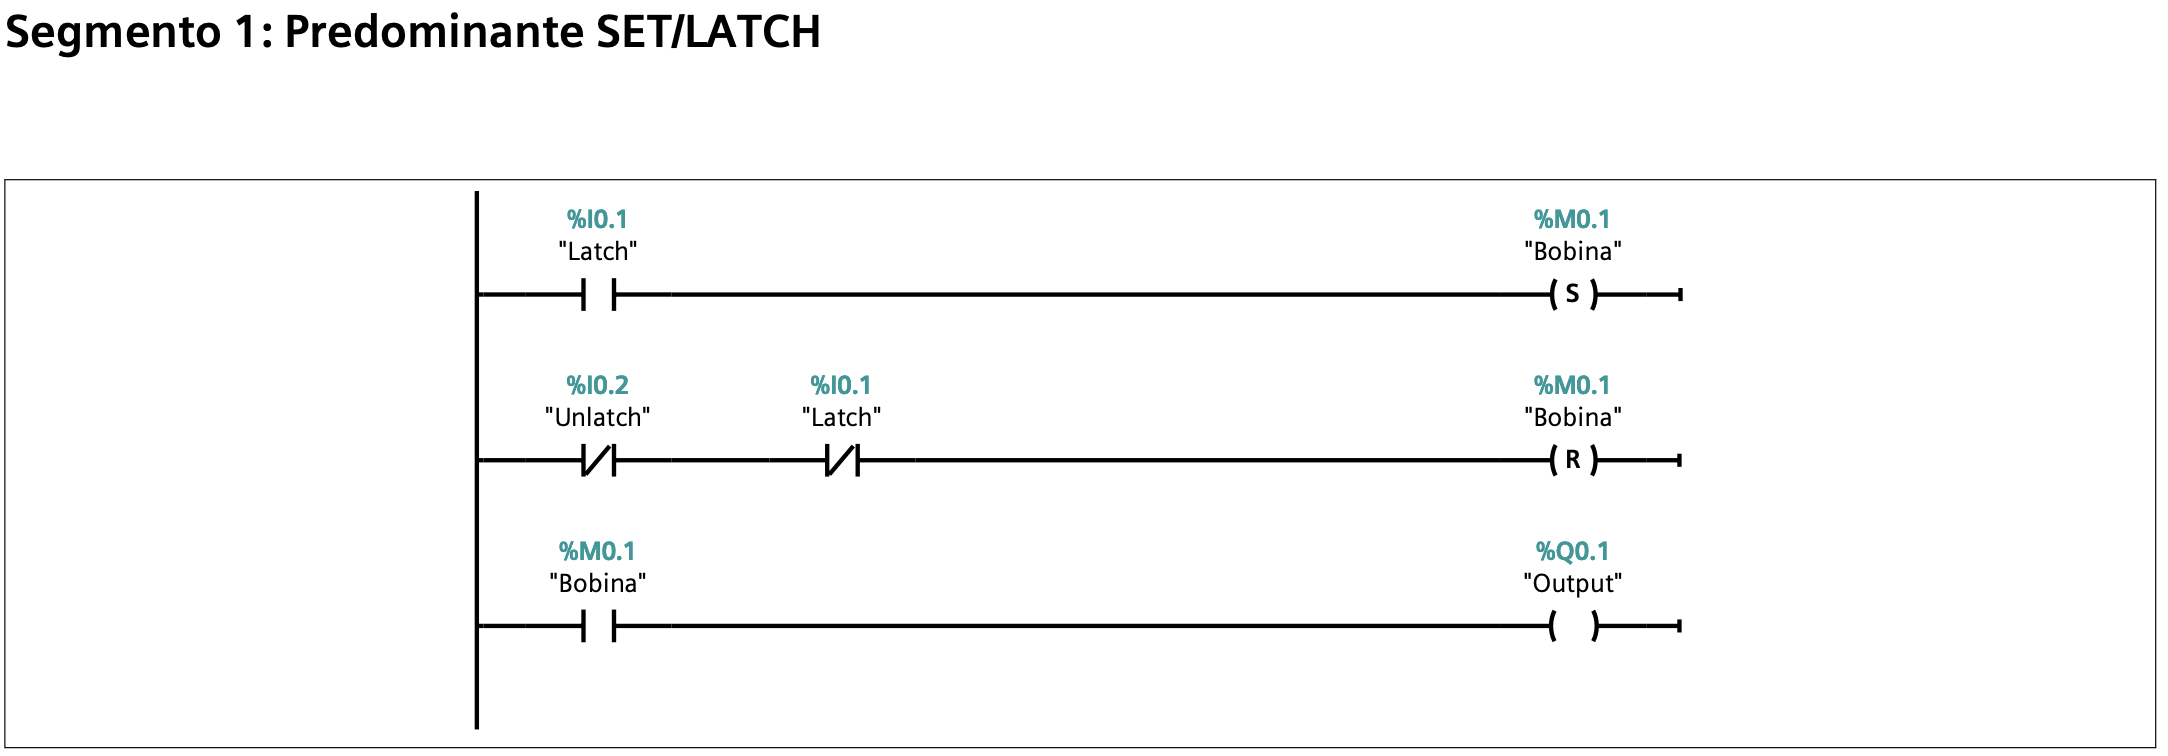
\includegraphics[width=1\textwidth]{screenshots/PredominanteSET.png}
          \caption{Circuito dominante SET}
          \label{fig:set}
        \end{figure}
  \item Creamos el segundo circuito dominante RESET.
        \begin{figure}[H]
          \centering
          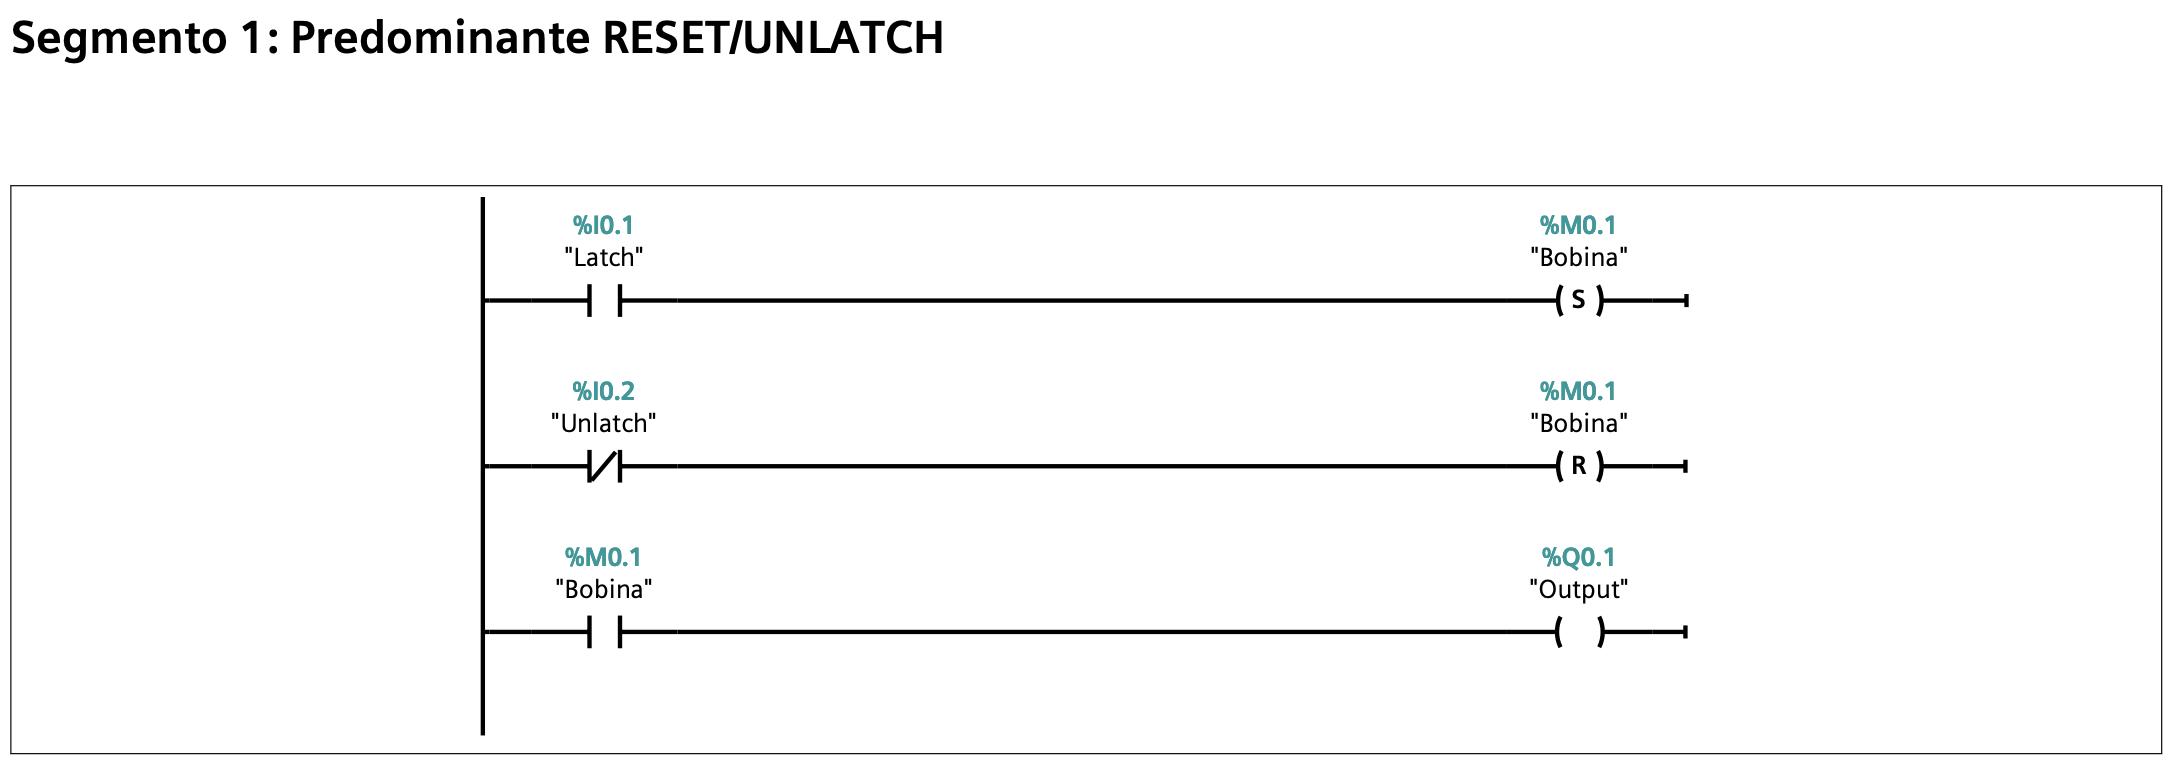
\includegraphics[width=1\textwidth]{screenshots/PredominanteRESET.png}
          \caption{Circuito dominante RESET}
          \label{fig:reset}
        \end{figure}
\end{enumerate}
\newpage

%----- CONCLUSIONES ----
\chapter{Conclusiones}
En esta práctica, se implementaron y simularon circuitos de control utilizando las funciones LATCH/UNLATCH, también conocidas como SET/RESET. A través de la creación de variables y la configuración adecuada de los componentes del circuito, se pudo verificar el funcionamiento de los circuitos predominantes SET y RESET.

El circuito predominante SET demostró ser efectivo para mantener una salida activada hasta que se cumpla una condición específica para desactivarla. Por otro lado, el circuito predominante RESET permitió desactivar una salida previamente activada por el circuito SET, asegurando que las operaciones se realicen de manera controlada y segura.
\newpage


\end{document}